\documentclass[10pt,leqno]{article}

\usepackage[%
  tmargin=1.2in,bmargin=1.2in,%
  lmargin=1.8in,rmargin=1.8in,%
]{geometry}
\usepackage{fancyhdr}
\usepackage{titlesec}
\usepackage{appendix}
\usepackage{microtype}
\usepackage[hyphens]{url}
\usepackage{enumitem}
\usepackage{xspace}
\usepackage{etoolbox}
\usepackage{ifthen}
\usepackage{tikz}
\usepackage{tikz-cd}

\usepackage{amsmath}
\definecolor{darkred}{rgb}{0.5,0.0,0.0}
\usepackage[%
  colorlinks,%
  linkcolor=darkred,%
  citecolor=darkred,%
  urlcolor=darkred,%
]{hyperref}
\usepackage{amsthm,amssymb}
% \usepackage[lining,semibold]{libertine}
% \usepackage{textcomp,stmaryrd}
% \usepackage[libertine,cmintegrals,bigdelims]{newtxmath}
% \useosf
% \usepackage[%
%   cal=boondox, calscaled=0.97,%
%   bb=boondox, bbscaled=0.98,%
% ]{mathalfa}
\usepackage{cleveref}

\frenchspacing
\urlstyle{rm}

\AtBeginDocument{%
  \setlength{\abovedisplayskip}{1.5ex plus 0.3ex minus 0.3ex}%
  \setlength{\abovedisplayshortskip}{1.0ex plus 0.3ex minus 0.3ex}%
  \setlength{\belowdisplayskip}{1.5ex plus 0.3ex minus 0.3ex}%
  \setlength{\belowdisplayshortskip}{1.0ex plus 0.3ex minus 0.3ex}%
}

\let\theoldbibliography\thebibliography
\renewcommand{\thebibliography}[1]{%
  \theoldbibliography{#1}%
  \setlength{\parskip}{0ex}
  \setlength{\itemsep}{0.5ex plus 0.2ex minus 0.2ex}
  \small
}

\pagestyle{fancy}
\renewcommand{\headrulewidth}{0pt}
\renewcommand{\footrulewidth}{0pt}
\fancyhf{}
\fancyfoot[C]{\small\thepage}

\renewcommand{\title}[1]{\newcommand{\thetitle}{#1}}
\renewcommand{\author}[1]{\newcommand{\theauthor}{#1}}
\renewcommand{\date}[1]{\newcommand{\thedate}{#1}}

\renewcommand{\maketitle}{%
  \begin{center}
    {\bfseries\MakeUppercase{%
      \thetitle}}\\[2.5ex]
    {\footnotesize\MakeUppercase{%
      \theauthor}}\\[2.5ex]
    \ifthenelse{\equal{\thedate}{}}{}{%
      \small%
      \setlength{\tabcolsep}{0.2em}%
      \begin{tabular}{rl}
        original: & \thedate \\
        updated: & \today
      \end{tabular}
    }
  \end{center}
  \vspace{2.5ex}
  \thispagestyle{fancy}
}

%%%%%%%%%%%%%%%%%%%%%%%%%%%%%%%%%%%%%%%%%%%%%%%%%%%%%%%%%%%%%%%%%%%%%%

\cspreto{section}{\setcounter{equation}{0}}

\titleformat{\section}{\centering\scshape}{\thesection.}{0.4em}{}
\titlespacing{\section}{0pt}{*4}{*1}
\titleformat{\subsection}{\scshape}{\thesubsection.}{0.4em}{}
\titlespacing{\subsection}{0pt}{*2.5}{*1}

% Display format for equations
\newcommand{\crefeqfmt}[1]{
  \crefformat{#1}{(##2##1##3)}
  \Crefformat{#1}{(##2##1##3)}
  \crefrangeformat{#1}{(##3##1##4--##5##2##6)}
  \Crefrangeformat{#1}{(##3##1##4--##5##2##6)}
  \crefmultiformat{#1}{(##2##1##3}{, ##2##1##3)}{, ##2##1##3}{, ##2##1##3)}
  \Crefmultiformat{#1}{(##2##1##3}{, ##2##1##3)}{, ##2##1##3}{, ##2##1##3)}
  \crefrangemultiformat{#1}{(##3##1##4--##5##2##6}{, ##3##1##4--##5##2##6)}{, ##3##1##4--##5##2##6}{, ##3##1##4--##5##2##6)}
  \Crefrangemultiformat{#1}{(##3##1##4--##5##2##6}{, ##3##1##4--##5##2##6)}{, ##3##1##4--##5##2##6}{, ##3##1##4--##5##2##6)}
}
% Display format for sections
\newcommand{\crefsecfmt}[1]{%
  \crefformat{#1}{\S##2##1##3}
  \Crefformat{#1}{\S##2##1##3}
  \crefrangeformat{#1}{\S\S##3##1##4--##5##2##6}
  \Crefrangeformat{#1}{\S\S##3##1##4--##5##2##6}
  \crefmultiformat{#1}{\S\S##2##1##3}{ and~##2##1##3}{, ##2##1##3}{ and~##2##1##3}
  \Crefmultiformat{#1}{\S\S##2##1##3}{ and~##2##1##3}{, ##2##1##3}{ and~##2##1##3}
  \crefrangemultiformat{#1}{\S\S##3##1##4--##5##2##6}{ and~##3##1##4--##5##2##6}{, ##3##1##4--##5##2##6}{ and~##3##1##4--##5##2##6}
  \Crefrangemultiformat{#1}{\S\S##3##1##4--##5##2##6}{ and~##3##1##4--##5##2##6}{, ##3##1##4--##5##2##6}{ and~##3##1##4--##5##2##6}
}
\crefeqfmt{equation}
\crefeqfmt{enumi}
\crefeqfmt{enumii}
\crefsecfmt{section}
\crefsecfmt{subsection}
\crefsecfmt{appendix}
\crefname{part}{Part}{Parts}
\crefname{chapter}{Chapter}{Chapters}
\crefname{figure}{Figure}{Figures}

\makeatletter

\newcommand{\thmnumfont}{\bfseries}
\newcommand{\thmheadfont}{\bfseries}
\newcommand{\thmnotefont}{\bfseries}
\newcommand{\thmhorizspace}{0.4em}

\def\swappedhead#1#2#3{%
  \thmnumber{\@upn{{\thmnumfont#2}}\@ifnotempty{#1}{.\hspace{0.25em}}}%
  \thmheadfont\thmname{#1}%
  \@ifnotempty{#3}{\ \thmnote{\thmnotefont(#3)}}%
}
\swapnumbers

\newtheoremstyle{block}%
  {2.0ex plus 0.2ex minus 0.1ex}% Space above
  {2.0ex plus 0.2ex minus 0.1ex}% Space below
  {} % Body font
  {} % Indent amount
  {\thmheadfont} % Theorem head font
  {.} % Punctuation after theorem head
  {\thmhorizspace} % Space after theorem head
  {} % Theorem head spec (can be left empty, meaning ‘normal’)

\renewenvironment{proof}[1][Proof]{\par
  \pushQED{\qed}%
  \normalfont%
  \topsep1ex plus 0.2ex minus 0.1ex\relax%
  \labelsep \thmhorizspace\relax%
  \trivlist
  \item[\hskip\labelsep\thmheadfont
    #1\@addpunct{.}]\ignorespaces
}{%
  \popQED\endtrivlist\@endpefalse%
}

\makeatother

\theoremstyle{block}

\newcommand{\defthm}[2]{%
  \newtheorem{#1}[equation]{#2}%
  \crefeqfmt{#1}%
  \newtheorem*{#1*}{#2}%
}

\defthm{algorithm}{Algorithm}
\defthm{conjecture}{Conjecture}
\defthm{construction}{Construction}
\defthm{convention}{Convention}
\defthm{corollary}{Corollary}
\defthm{definition}{Definition}
\defthm{definitions}{Definitions}
\defthm{example}{Example}
\defthm{examples}{Examples}
\defthm{exercise}{Exercise}
\defthm{fact}{Fact}
\defthm{intuition}{Intuition}
\defthm{lemma}{Lemma}
\defthm{notation}{Notation}
\defthm{nothing}{}
\defthm{proposition}{Proposition}
\defthm{question}{Question}
\defthm{remark}{Remark}
\defthm{remarks}{Remarks}
\defthm{situtation}{Situation}
\defthm{theorem}{Theorem}

\setlist{%
  leftmargin=2.5em, parsep=0ex, listparindent=\parindent,
  itemsep=1.0ex, topsep=1.0ex,%
}

\setlist[enumerate, 1]{%
  label=(\alph*),%
  ref=\alph*,%
  widest=d,%
}
\setlist[enumerate, 2]{%
  label=(\roman*),%
  ref=\theenumi.\roman*,%
}
\setlist[itemize, 1]{%
  label=$\vcenter{\hbox{\footnotesize$\bullet$}}$,%
}
\setlist[itemize, 2]{label=--}

%%%%%%%%%%%%%%%%%%%%%%%%%%%%%%%%%%%%%%%%%%%%%%%%%%%%%%%%%%%%%%%%%%%%%%

\makeatletter

\let\ea\expandafter

\newcount\foreachcount

\def\foreachletter#1#2#3{\foreachcount=#1
  \ea\loop\ea\ea\ea#3\@alph\foreachcount
  \advance\foreachcount by 1
  \ifnum\foreachcount<#2\repeat}

\def\foreachLetter#1#2#3{\foreachcount=#1
  \ea\loop\ea\ea\ea#3\@Alph\foreachcount
  \advance\foreachcount by 1
  \ifnum\foreachcount<#2\repeat}

% Roman: \rA is \mathrm{A}
\def\definerm#1{%
  \ea\gdef\csname r#1\endcsname{\ensuremath{\mathrm{#1}}\xspace}}
\foreachLetter{1}{27}{\definerm}
\foreachletter{1}{27}{\definerm}
% Script: \sA is \mathscr{A}
\def\definescr#1{%
  \ea\gdef\csname s#1\endcsname{\ensuremath{\mathscr{#1}}\xspace}}
\foreachLetter{1}{27}{\definescr}
% Calligraphic: \cA is \mathcal{A}
\def\definecal#1{%
  \ea\gdef\csname c#1\endcsname{\ensuremath{\mathcal{#1}}\xspace}}
\foreachLetter{1}{27}{\definecal}
% Bold: \bA is \mathbf{A}
\def\definebold#1{%
  \ea\gdef\csname b#1\endcsname{\ensuremath{\mathbf{#1}}\xspace}}
\foreachLetter{1}{27}{\definebold}
% Blackboard Bold: \lA is \mathbb{A}
\def\definebb#1{%
  \ea\gdef\csname l#1\endcsname{\ensuremath{\mathbb{#1}}\xspace}}
\foreachLetter{1}{27}{\definebb}
% Fraktur: \ka is \mathfrak{a}, \kA is \mathfrak{A}
\def\definefrak#1{%
  \ea\gdef\csname k#1\endcsname{\ensuremath{\mathfrak{#1}}\xspace}}
\foreachletter{1}{27}{\definefrak}
\foreachLetter{1}{27}{\definefrak}
% Sans serif: \iA \is \mathsf{A}
\def\definesf#1{%
  \ea\gdef\csname i#1\endcsname{\ensuremath{\mathsf{#1}}\xspace}}
\foreachletter{1}{6}{\definesf}
\foreachletter{7}{14}{\definesf}
\foreachletter{15}{27}{\definesf}
\foreachLetter{1}{27}{\definesf}
% Bar: \Abar is \overline{A}, \abar is \overline{a}
\def\definebar#1{%
  \ea\gdef\csname #1bar\endcsname{\ensuremath{\overline{#1}}\xspace}}
\foreachLetter{1}{27}{\definebar}
\foreachletter{1}{8}{\definebar} % \hbar is something else!
\foreachletter{9}{15}{\definebar} % \obar is something else!
\foreachletter{16}{27}{\definebar}
% Tilde: \Atil is \widetilde{A}, \atil is \widetilde{a}
\def\definetil#1{%
  \ea\gdef\csname #1til\endcsname{\ensuremath{\widetilde{#1}}\xspace}}
\foreachLetter{1}{27}{\definetil}
\foreachletter{1}{27}{\definetil}
% Hats: \Ahat is \widehat{A}, \ahat is \widehat{a}
\def\definehat#1{%
  \ea\gdef\csname #1hat\endcsname{\ensuremath{\widehat{#1}}\xspace}}
\foreachLetter{1}{27}{\definehat}
\foreachletter{1}{27}{\definehat}
% Checks: \Achk is \widecheck{A}, \achk is \widecheck{a}
\def\definechk#1{%
  \ea\gdef\csname #1chk\endcsname{\ensuremath{\widecheck{#1}}\xspace}}
\foreachLetter{1}{27}{\definechk}
\foreachletter{1}{27}{\definechk}
% Underline: \Aund is \underline{A}, \aund is \underline{a}
\def\defineul#1{%
  \ea\gdef\csname #1und\endcsname{\ensuremath{\underline{#1}}\xspace}}
\foreachLetter{1}{27}{\defineul}
\foreachletter{1}{27}{\defineul}

\makeatother

%%%%%%%%%%%%%%%%%%%%%%%%%%%%%%%%%%%%%%%%%%%%%%%%%%%%%%%%%%%%%%%%%%%%%%

\usetikzlibrary{calc,decorations.pathmorphing,shapes,arrows}
\tikzcdset{
  arrow style=tikz,
  diagrams={>={stealth}},
}

\newcommand{\arrlen}{1em}
\renewcommand{\to}{\mathrel{\tikz[baseline]%
    \draw[>=stealth,->](0,0.5ex)--(\arrlen,0.5ex);}}
\newcommand{\from}{\mathrel{\tikz[baseline]%
    \draw[>=stealth,<-](0,0.5ex)--(\arrlen,0.5ex);}}
\renewcommand{\mapsto}{\mathrel{\tikz[baseline]%
    \draw[>=stealth,|->](0,0.5ex)--(\arrlen,0.5ex);}}
\newcommand{\inj}{\mathrel{\tikz[baseline]%
    \draw[>=stealth,right hook->](0,0.5ex)--(\arrlen,0.5ex);}}
\newcommand{\surj}{\mathrel{\tikz[baseline]%
    \draw[>=stealth,->>](0,0.5ex)--(\arrlen,0.5ex);}}
\newcommand{\fromto}{\mathrel{%
  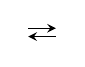
\begin{tikzpicture}[baseline]%
    \draw[>=stealth,<-](0,0.15ex)--(\arrlen,0.15ex);%
    \draw[>=stealth,->](0,0.85ex)--(\arrlen,0.85ex);%
  \end{tikzpicture}}}
\newcommand{\doubto}{\mathrel{%
  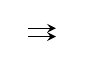
\begin{tikzpicture}[baseline]%
    \draw[>=stealth,->](0,0.15ex)--(\arrlen,0.15ex);%
    \draw[>=stealth,->](0,0.85ex)--(\arrlen,0.85ex);%
  \end{tikzpicture}}}
\newcommand{\lblto}[1]{\mathrel{%
    \begin{tikzpicture}[baseline= {( $ (current bounding box.south) + (0,-0.5ex) $ )}]
      \node[inner sep=.4ex] (a) {\,$\scriptstyle #1$\,};
      \draw[>=stealth,->] (a.south west) -- (a.south east);
    \end{tikzpicture}}}
\newcommand{\isoto}{\lblto{\sim}}

\newcommand{\simpl}[3]{
  \begin{tikzcd}[ampersand replacement=\&, column sep=small]
    #1 \&
    #2 \ar[l, shift right=0.35ex]
       \ar[l, shift left=0.35ex] \&
    #3 \ar[l, shift right=0.70ex]
       \ar[l, shift left=0.70ex]
       \ar[l] \&
    \cdots \ar[l, shift right=0.35ex]
           \ar[l, shift left=0.35ex]
           \ar[l, shift right=1.05ex]
           \ar[l, shift left=1.05ex]
  \end{tikzcd}
}
\newcommand{\cosimpl}[3]{
  \begin{tikzcd}[ampersand replacement=\&, column sep=small]
    #1 \ar[r, shift right=0.35ex]
       \ar[r, shift left=0.35ex] \&
    #2 \ar[r, shift right=0.70ex]
       \ar[r, shift left=0.70ex]
       \ar[r] \&
    #3 \ar[r, shift right=0.35ex]
       \ar[r, shift left=0.35ex]
       \ar[r, shift right=1.05ex]
       \ar[r, shift left=1.05ex] \&
    \cdots
  \end{tikzcd}
}

\newcommand{\tto}{\mathrel{\tikz[baseline]%
    \draw[>=stealth,->,double, double distance = 0.3ex](0,0.5ex)--(\arrlen,0.5ex);}}
\newcommand{\doubfrom}{\mathrel{%
  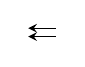
\begin{tikzpicture}[baseline]%
    \draw[>=stealth,<-](0,0.15ex)--(\arrlen,0.15ex);%
    \draw[>=stealth,<-](0,0.85ex)--(\arrlen,0.85ex);%
  \end{tikzpicture}}}
\newcommand{\tripfrom}{\mathrel{%
  
\begin{tikzpicture}[baseline]%
    \draw[>=stealth,<-](0,0.00ex)--(\arrlen,0.00ex);%
    \draw[>=stealth,<-](0,0.50ex)--(\arrlen,0.50ex);%
    \draw[>=stealth,<-](0,1.00ex)--(\arrlen,1.00ex);%
  \end{tikzpicture}}}


\renewcommand{\l}{\left}
\renewcommand{\r}{\right}
\newcommand{\f}{\frac}
\renewcommand{\o}{\overline}
\renewcommand{\u}{\underline}
\newcommand{\til}{\widetilde}
\renewcommand{\hat}{\widehat}
\newcommand{\del}{\partial}
\newcommand{\dash}{\text{-}}
\renewcommand{\c}{\colon}
\newcommand{\lc}{\,:\!}
\newcommand{\ce}{\coloneq}%{\mathrel{:=}}
\newcommand{\ec}{\eqcolon}%{\mathrel{=:}}
\newcommand{\iso}{\simeq}
\newcommand{\dual}{\vee}
\newcommand{\ldb}{\llbracket}
\newcommand{\rdb}{\rrbracket}

\newcommand{\Obj}{\operatorname{Obj}}
\newcommand{\Hom}{\operatorname{Hom}}
\newcommand{\Map}{\operatorname{Map}}
\newcommand{\Fun}{\operatorname{Fun}}
\newcommand{\Aut}{\operatorname{Aut}}
\newcommand{\Iso}{\operatorname{Iso}}
\renewcommand{\id}{\mathrm{id}}
\renewcommand{\im}{\operatorname{im}}
\newcommand{\op}{\mathrm{op}}
\newcommand{\univ}{\mathrm{univ}}
\newcommand{\colim}{\operatorname*{colim}}
\newcommand{\dlim}{\displaystyle\lim}
\newcommand{\dcolim}{\displaystyle\colim}
\newcommand{\Spec}{\operatorname{Spec}}
\newcommand{\Spf}{\operatorname{Spf}}

%%%%%%%%%%%%%%%%%%%%%%%%%%%%%%%%%%%%%%%%%%%%%%%%%%%%%%%%%%%%%%%%%%%%%%


\title{Math 216A Homework 9}
\author{Arpon Raksit}
\date{December 1, 2016}

\numberwithin{block}{section}

%%%%%%%%%%%%%%%%%%%%%%%%%%%%%%%%%%%%%%%%%%%%%%%%%%%%%%%%%%%%%%%%%%%%%%

\begin{document}
\maketitle


%%%%%%%%%%%%%%%%%%%%%%%%%%%%%%%%%%%%%%%%%%%%%%%%%%%%%%%%%%%%%%%%%%%%%%

\section{Geometric connectedness}

\begin{nothing}
  \label{pointset}

  Let $\pi \c Y \to X$ be a map of topological spaces. Let $\sC_X,\sC_Y$ denote the sets of connected components in $X,Y$. Note that since images of connected spaces are connected, $\pi$ induces a map of sets $\pi_* \c \sC_Y \to \sC_X$.

  \begin{sublemma}
    \label{pointset-component-bijection}
    Suppose that for any connected component $C$ of $X$ the preimage $\pi^{-1}(C)$ is connected. Then $\pi_* \c \sC_Y \to \sC_X$ is a bijection.

    \begin{proof}
      In this case, taking preimages defines a two-sided inverse $\pi^{-1} \c \sC_X \to \sC_Y$ to $\pi_*$.
    \end{proof}
  \end{sublemma}

  \begin{sublemma}
    \label{pointset-connected-fibers}
    Suppose that:
    \begin{enumerate}
    \item $\pi$ is open or closed; 
    \item the fibers of $\pi$ are connected (in particular nonempty, so $\pi$ is surjective). 
    \end{enumerate}
    Then $\pi_* \c \sC_Y \to \sC_X$ is a bijection.

    \begin{proof}
      By \cref{pointset-component-bijection} it suffices to show that the preimage of any connected component $C$ of $X$ is connected. Thus we may reduce to the case that $X$ is connected, where we want to show $Y$ is connected.

      Suppose not: then we may write $Y = A \amalg B$ with $A,B$ nonempty and clopen subspaces of $Y$. Since $\pi$ is surjective we have $X = \pi(A) \cup \pi(B)$. Since $X$ is connected, and $\pi$ is open or closed, $\pi(A)$ and $\pi(B)$ cannot be disjoint; thus we may choose $x \in \pi(A) \cap \pi(B)$. That means the fiber $Y_x$ meets both $A$ and $B$, and hence $Y_x = (A \cap Y_x) \amalg (B \cap Y_x)$ is disconnected. This proves the claim.
    \end{proof}
  \end{sublemma}
\end{nothing}

\begin{proposition}
  \label{alg-closed-connected}
  Let $X$ be a scheme over an algebraically closed field $k$. Let $K/k$ be an extension field, and let $X_K \ce X \times_k K$ be the base-change. Then the projection $\pi \c X_K \to X$ induces a bijection on connected components; in particular, $X_K$ is connected if and only if $X$ is connected.

  \begin{proof}
    By exercise 2(iv) the map $\pi \c X_K \to X$ is open. So by \cref{pointset-connected-fibers} it suffices to show the fibers of $\pi$ are connected.

    Pick any point $x \in X$, and consider the canonical map $\Spec(\kappa(x)) \to X$. The fiber of $X_K$ over $x$ is given by
    \[
      X_K \times_X \Spec(\kappa(x)) \iso \Spec(K) \times_{\Spec(k)} X \times_X \Spec(\kappa(x)) \iso \Spec(K \otimes_k \kappa(x)).
    \]
    In homework 1 we proved that, since $k$ is algebraically closed, $K \otimes_k \kappa(x)$ is a domain; hence its spectrum is connected.
  \end{proof}
\end{proposition}

\begin{proposition}
  \label{geom-alg-closed}
  Let $X$ be a scheme over a field $k$. The following are equivalent:
  \begin{enumerate}
  \item \label{geom-alg-closed-geom} The base-change $X_K \ce X \times_k K$ is connected for every extension $K/k$.
  \item \label{geom-alg-closed-alg-closed} The base-change $X_{\kbar} \ce X \times_k \kbar$ is connected, where $\kbar$ is any algebraic closure of $k$.
  \end{enumerate}

  \begin{proof}
    \cref{geom-alg-closed-geom} $\shimplies$ \cref{geom-alg-closed-alg-closed}: Tautological.

    \cref{geom-alg-closed-alg-closed} $\shimplies$ \cref{geom-alg-closed-geom}:  Let $K/k$ be any extension. Let $\kbar$ and $\Kbar$ be algebraic closures of $k$ and $K$. The canonical map
    \[
      X_{\Kbar} \ce X \times_k \Kbar \iso X_K \times_K \Kbar \to X_K
    \]
    is surjective, so it suffices to show $X_{\Kbar}$ is connected. We may embed $\kbar$ as a subextension of $\Kbar/k$, and then we're done by \cref{alg-closed-connected}.
  \end{proof}
\end{proposition}

\begin{proposition}
  \label{rational-connected}
  Let $X$ be a scheme over a field $k$. Suppose $X$ has a $k$-rational point. Let $K/k$ be an extension field. If $X$ is connected, then the base change $X_K \ce X \times_k K$ is connected.

  \begin{proof}
    By \cref{geom-alg-closed} we may reduce to the case $K = \kbar$. Suppose $X_K = X_{\kbar}$ is not connected, so we may write $X_K = A \amalg B$ for $A,B$ nonempty clopen subspaces. Let $\pi \c X_K \to X$ be the projection. Let $x \c \Spec k \to X$ be a $k$-rational point, and observe that the fiber $(X_K)_x$ is
    \[
      X_K \times_X \Spec(k) \iso \Spec(K) \times_{\Spec(k)} X \times_X \Spec(k) \iso \Spec(K),
    \]
     hence is a single point $x' \in X_K$. Without loss of generality suppose $x' \in A$, so $x' \notin B$, and hence (by the above computation of the fiber) $\pi(B)$ does not contain $x$ and hence is a proper nonempty subspace of $X$. But now, as $\Spec(K) = \Spec(\kbar) \to \Spec(k)$ is an integral map, so is its base change $\pi \c X_K \to X$, so $\pi$ is closed. And by exercise 2(iv), $\pi$ is open. Thus $B$ being clopen implies $\pi(B)$ is clopen, and hence $X$ is also not connected.
  \end{proof}
\end{proposition}

\begin{proposition}
  \label{geom-connected}
  Let $X$ be a scheme locally of finite type over a field $k$. Suppose $X \times_k L$ is connected for all finite separable extensions $L/k$. Then $X \times_k K$ is connected for all extensions $K/k$.

  \begin{proof}
    By \cref{geom-alg-closed} it suffices to show $X \times_k \kbar$ is connected. Since $X$ is locally of finite type over $k$, it has a closed point $x$, and moreover $\kappa(x)/k$ is a finite extension. Then $X \times_k \kappa(x)$ is a scheme over $\kappa(x)$ with a $\kappa(x)$-rational point, and we may embed $\kappa(x)$ in $\kbar$, so by \cref{rational-connected} it suffices to show $X \times_k \kappa(x)$ is connected. Let $L/k$ be the maximal separable subextension of $\kappa(x)$. Then $\kappa(x)/L$ is purely inseparable, so $\Spec(\kappa(x)) \to \Spec(L)$ is a universal homeomorphism, and thus $X \times_k \kappa(x)$ is homeomorphic to $X \times_k L$, which is connected by hypothesis, finishing the proof.
  \end{proof}
\end{proposition}

%%%%%%%%%%%%%%%%%%%%%%%%%%%%%%%%%%%%%%%%%%%%%%%%%%%%%%%%%%%%%%%%%%%%%%

\end{document}
